% === [ Design ] ===============================================================

\section{Design}

% TODO: Add design notes
%    - The LLVM IR libraries are developed as reusable components for compilers, decompilers, and other semantic analysis tools. They aim to support generic semantic analysis applications, while satisfying the explicit requirements [1] of the third party llgo compiler.
%
% [1]: https://github.com/go-llvm/llvm/issues/40

% TODO: Add
%   - A decompilation system composed of individual components and based on the principle of separation of concerns.
%   - The system must be language-agnostic so that decompilation passes can be reused from other programming language environments.

foo

% --- [ Programming Language Considerations ] ----------------------------------

\subsection{Programming Language Considerations}

% TODO: Move the "Ideomatic Coding" section here? Adapt its text to fit the Design section. Choice of section title?

% TODO: Clarify the benefits and drawbacks of using Go over C++ which would be the obvious choice for LLVM IR heavy projects. Choosing not to use C++ validates the language-agnostic aspects of the design.
% - Compilation speed. ll2dot takes > 1.5m whereas a regular Go program takes < 1s.

% TODO: Mention software composition.

% TODO: Add and tie in to the pragmatic aspects of Go?
%    * tooling?
%       - "go get" can locate all dependencies.
%       - compilation time is linear rather than exponential with regards to dependencies.
%    * automation?

foo

% --- [ Decompiler Pipeline ] --------------------------------------------------

\subsection{Decompiler Pipeline}

% TODO: Describe where the "restructure" component fits in the overall decompilation pipeline. Mention which projects and tools that may be used to fill the gaps. bin_descend and IDA python script of MC-Semantics -> Google Protocol Buffer -> cfg_to_bc -> LLVM IR

% TODO: Rewrite and clarify.

The decompilation pipeline is made of up several components which are conceptually grouped into three modules. The front-end module translates a variety of inputs (such as binary files and source code) into LLVM IR by utilizing a collection of tools developed by several independent open source projects. The middle-end lifts the LLVM IR to a high-level representation by conducting a control flow analysis which generates a structured CFG of each function. The back-end generates high-level control flow primitives such as if-statements and for-loops based on the structured CFG. In addition it translates the individual instructions of the LLVM IR to expressions and statements of the target programming language (in this case Go). The interaction between the front-end, middle-end and back-end modules is visualized in \cref{fig:decompilation_pipeline}.

% * Front-end
%    - binary -> LLVM IR ([MC-Semantics](https://github.com/trailofbits/mcsema), [Dagger](http://dagger.repzret.org/) or [Fracture](https://github.com/draperlaboratory/fracture))
%    - source code -> LLVM IR (clang, ghc, rustc, ...)
% * Middle-end
%    - LLVM IR -> Unstructured CFG ([ll2dot](https://github.com/mewrev/ll2dot))
%    - Unstructured CFG -> Structured CFG ([iso](https://github.com/mewrev/graphs) and [merge](https://github.com/mewrev/graphs).)
%       + Truthfully `ll2go` doesn't make direct use of `iso` or `merge` but rather the graph libraries. A future ambition is to allow `iso` and `merge` to output JSON such that they may be used directly by `ll2go`.
% * Back-end
%    - Structured CFG -> Go ([ll2go](https://github.com/mewrev/ll2go))


\begin{figure}[htbp]
	\begin{center}
		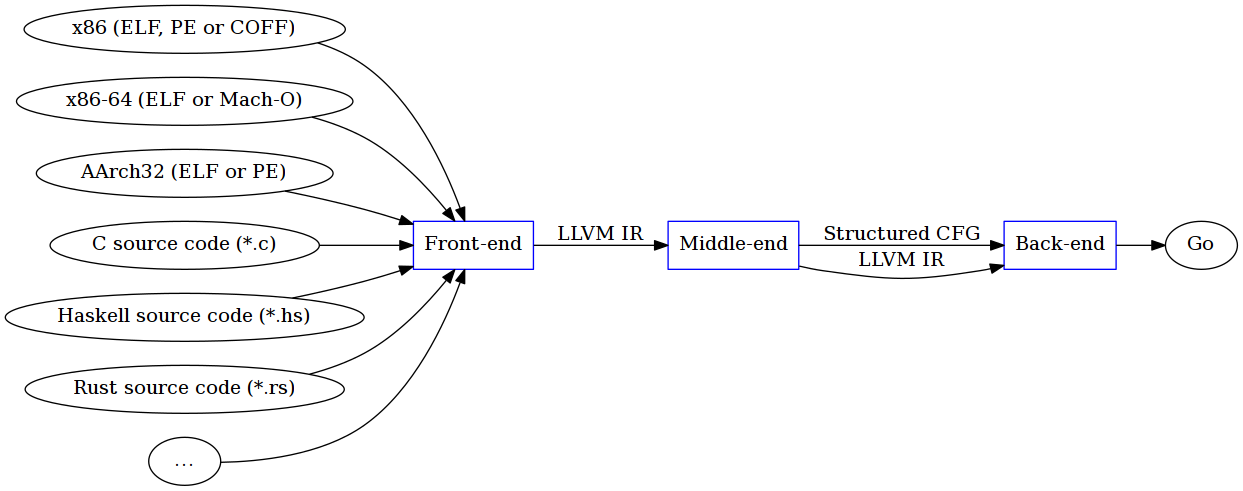
\includegraphics[width=\textwidth]{inc/decompilation_pipeline.png}
		\caption{foo}
		\label{fig:decompilation_pipeline}
	\end{center}
\end{figure}


\subsubsection{Front-end}

% TODO: Rewrite and clarify.

The front-end module is responsible for converting the input into LLVM IR. Two common scenarios exists, converting binary files (e.g. executables, shared libraries and relocatable object code) and converting source code (e.g. C, Haskell, Rust, …) into LLVM IR. The first scenario is presented in \cref{fig:front-end_binary} and the second in \cref{fig:front-end_source}.

% TODO: Mention opt --mem2reg.

\begin{figure}[htbp]
	\begin{center}
		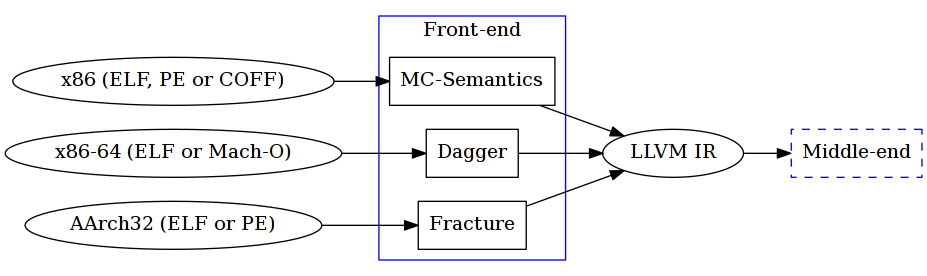
\includegraphics[width=\textwidth]{inc/front-end_binary.png}
		\caption{foo}
		\label{fig:front-end_binary}
	\end{center}
\end{figure}

\begin{figure}[htbp]
	\begin{center}
		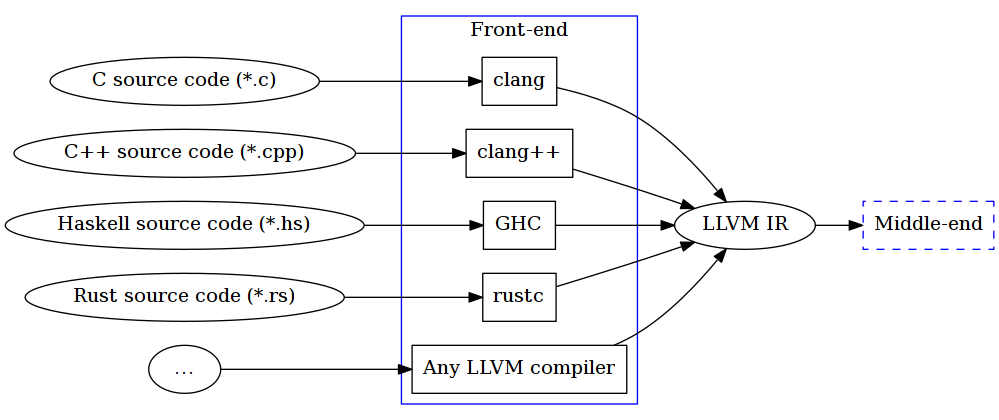
\includegraphics[width=\textwidth]{inc/front-end_source.png}
		\caption{foo}
		\label{fig:front-end_source}
	\end{center}
\end{figure}

\subsubsection{Middle-end}

% TODO: Rewrite and clarify.

% TODO: Create a restructure tool which replaces the use of iso.

The middle-end is responsible for lifting the LLVM IR to a high-level representation through a series of decompilation passes. The \texttt{ll2dot} tool generates a CFG (in the DOT file format) for each function of a given LLVM IR input file. The \texttt{iso} tool searches for subgraph isomorphisms of control flow primitives in a given CFG. Once located the nodes identified subgraph are merged into a single node which is labeled with the high-level control flow primitive. Successive iterations continue to simplify the CFG until only one node is left, at which point the high-level control flow structure has been recovered. Should the \texttt{iso} tool fail to reduce the graph into a single node, the graph is considered irreducible with regards to the supported high-level control flow primitives. The interaction between the front-end, the \texttt{ll2dot} and \texttt{iso} tools of the middle-end and the back-end is illustrated in \cref{fig:middle-end}.

\begin{figure}[htbp]
	\begin{center}
		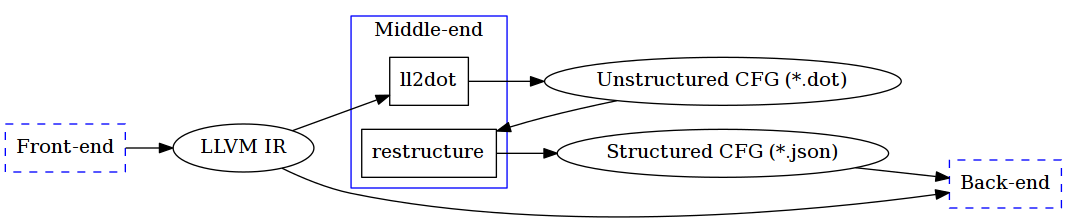
\includegraphics[width=\textwidth]{inc/middle-end.png}
		\caption{foo}
		\label{fig:middle-end}
	\end{center}
\end{figure}

\subsubsection{Back-end}

% TODO: Rewrite and clarify.

% TODO: Add ref to rsc's grind tool.

% TODO: Proof-of-concept. Implement a back-end for another language and written in another language. This would stress test the language-agnostic aspects of the design, thus making sure that the heavy-lifting is done in the middle-end and not in ll2go.

The back-end is responsible for translating the structured control flow graph of the LLVM IR into a target programming language. The \texttt{ll2go} tool is a proof of concept back-end which produces unpolished Go source code. The polishing is done by separate tools which fixes potential compilation issues and makes the code more idiomatic. The interaction between the middle-end and the back-end is illustrated in \cref{fig:back-end}. Currently the \texttt{ll2gofix} replaces return-statements in the \texttt{main} function with calls to \texttt{os.Exit}, which is required since the \texttt{main} function has no return arguments in Go. Instead the Go runtime calls \texttt{os.Exit} with the status-code \texttt{0} once \texttt{main} returns to signal successful termination. This eliminates the need to always end the \texttt{main} function with a \texttt{return 0;} statement as is common practise in C. A future ambition is to make use of and possibly contribute to the \texttt{grind} tool which moves variable declarations closer to their usage, and thus improving readability of the code. Generally the aim is to keep the \texttt{ll2go} tool as simple as possible. The middle-end is responsible for the structural analysis, and as a future ambition the data flow analysis. Since the complexity of the back-end is kept to a minimum it should be trivial to implement support for other output languages.

\begin{figure}[htbp]
	\begin{center}
		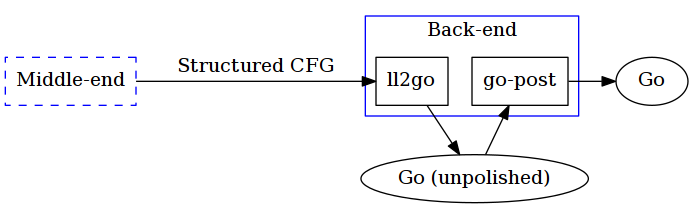
\includegraphics[width=\textwidth]{inc/back-end.png}
		\caption{foo}
		\label{fig:back-end}
	\end{center}
\end{figure}

% --- [ System Architecture ] --------------------------------------------------

\subsection{System Architecture}

% TODO: Visualize the dependency graph of the "restructure" tool and describe in detail what input it expects and what output it produces.

% TODO: Write about. Input and output LLVM IR to operate well with components written in other languages. Output LLVM IR with information about high-level control structures stored in the basic block names or in metadata.

foo

% TODO: Mention package division.

\subsection{Data-driven Design}

% TODO: Mention: CFG invariants (e.g. single-entry, single-exit)

% TODO: Add notes about the use of DOT-files to describe control flow primitives. Think if and how this could be pushed further to facilitate the development of future back-ends.

\subsection{Limitations}

% TODO: Add limitations related to the design choices. Which limitations are easily solvable given more time and which are fundamentally part of the design.
%    - No support for n-way conditionals (e.g.switch-statements).

foo

% --- [ Security Assessment ] --------------------------------------------------

\subsection{Security Assessment}

To assess the security of the decompiler pipeline, lets imagine a scenario in which users are given access to the implementation details and source code of the entire system and may provide arbitrary input to any of its components. A potential scenario could involve a web site which provides decompilation as a service and allows its users to interact with the various stages of the decompiler pipeline. The Retargetable Decompiler (see \cref{sec:retargetable_decompiler}) provides such a service, except it only allows users to interact with the binary analysis stage of the pipeline (see \cref{sec:binary_analysis}) and its source code is proprietary. The scope of this security assessment will be limited to the various components of the decompiler pipeline and their interaction. In particular security issues related to the operating system, network stack, web server and web site (e.g. SQL-injection and XSS vulnerabilities) of the decompilation service are intentionally excluded from the scope of the security assessment.

The objective of an attacker may be to escalate their privileges in a system by exploiting it to execute actions not intended by design. Since the security of any system is only as strong as its weakest link, it is critical to identify and isolate likely targets for attacks. Projects which consist of or depend on large C or C++ code bases may exhibit memory safety issues, such as buffer overflows or use-after-free vulnerabilities. These issues are considered low-hanging fruit for attackers and have a long history of successful exploitation \cite{for_fun_and_profit}. Several modern programming languages (including Go) provide memory safety guarantees and may solve these issues by inserting bounds-checking for array accesses and using garbage collection for memory management. Code written in memory safe languages may still contain other security vulnerabilities caused by logic errors or insufficient validation, sanitation and parametrization of input (e.g. command injection and directory traversal vulnerabilities).

The number of lines of code in a project may give an indication to the project's complexity and to some extent its potential attack surface. As summarized in \cref{tbl:loc_summary} every component of the decompiler pipeline except \texttt{iso} depends on LLVM. The LLVM code base contains approximately \numprint{800000} lines of C++ source code, and even if only a portion of the code will be linked into the executables it is an interesting target for attacks. One thing to keep in mind is that there are several high-end users of the LLVM project (such as Apple, Intel, NVIDIA and Sony \cite{llvm_users}) and it has a well established code reviewing process. Some of the LLVM developers are also very well educated in common security vulnerabilities and have developed the Clang Static Analyzer, which is a static source code analysis tool that locates bugs (such as buffer overflows and use-after-free issues) in C and C++ programs \cite{clang_analyzer}. The LLVM project may contain several security issues due to its size, but they are most likely difficult to discover since the low-hanging fruit have been caught already by the Clang Static Analyzer. Similarly, Google Protocol Buffers are used extensively by several companies and organizations and the likelyhood of discovering a simple security vulnerability in its code base is low.

\begin{table}[htbp]
	\begin{center}
		\begin{tabular}{|l|l|l|l|}
			\hline
			\textbf{Project} & \textbf{Language} & \textbf{Lines} & \textbf{Dependencies} \\
			\hline
			\multicolumn{4}{|l|}{\hspace{4ex} \textit{Front-end}} \\
			\hline
			Dagger & C++ & \numprint{2000} & LLVM \\
			Fracture & C++ & \numprint{20000} & LLVM \\
			MC-Semantics & C++ & \numprint{25000} & LLVM and Google Protocol Buffers \\
			\hline
			\multicolumn{4}{|l|}{\hspace{4ex} \textit{Middle-end}} \\
			\hline
			ll2dot & Go & \numprint{500} & LLVM and dot \\
			iso & Go & \numprint{2000} & dot \\
			\hline
			\multicolumn{4}{|l|}{\hspace{4ex} \textit{Back-end}} \\
			\hline
			ll2go & Go & \numprint{1500} & LLVM, llvm (Go), iso and dot \\
			\hline
			\multicolumn{4}{|l|}{\hspace{4ex} \textit{Dependencies}} \\
			\hline
			LLVM & C++ & \numprint{800000} & - \\
			Google Protocol Buffers & C++ & \numprint{125000} & - \\
			llvm (Go) & Go & \numprint{5000} & - \\
			dot & Go & \numprint{7000} & - \\
			\hline
		\end{tabular}
	\end{center}
	\caption{A rough summary of each project specifying their programming language, number of lines of code and dependencies.}
	\label{tbl:loc_summary}
\end{table}

There are still three potential targets which may contain memory related vulnerabilities, namely the front-end projects which translate binary executables, object code and shared libraries to LLVM IR.

% easy to make mistakes in the parsing logic. Trust header fields without verifying.

% TODO: Mention the unnamed hack (gain access to the names of anonymous basic blocks).
%    - Unable to trust the integrity of the output of local files are tampered with. Trusting trust.

% TODO: Security through obscurity
% TODO: Defence in depth
%    - Use several layers of security such that one may fail without disrupting the integrity of the entire system (e.g. jail [chroot on steroids])
% TODO: Memory Safety
%    - Mitigated using security through obscurity (e.g. ASLR, ) and true security (e.g. W^X).
